\documentclass[crop,tikz]{standalone}

\tikzset{>=latex}
\usetikzlibrary{decorations.markings}
\colorlet{green}{black!40!green}
\newcommand{\place}{\vec{r}}
\newcommand{\velocity}{\vec{v}}

\begin{document}
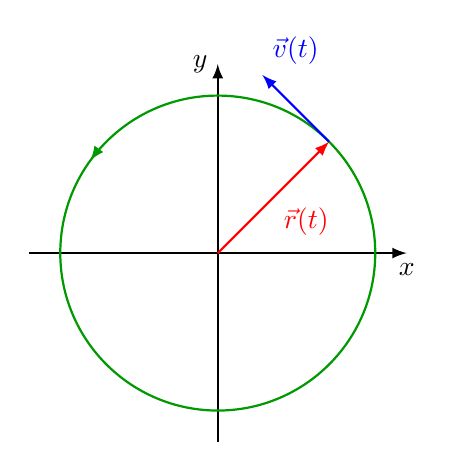
\begin{tikzpicture}[scale=2]
    \draw[->,thick] (-1.2,0) -- (1.2,0) node[below] {$x$};
    \draw[->,thick] (0,-1.2) -- (0,1.2) node[left] {$y$};
    \draw[
      decoration={markings, mark=at position 0.4 with {\arrow{>}}},
      postaction={decorate},
      green,
      thick
    ] (0,0) circle (1);
    \draw[->,thick,red] (0,0) -- node[right,anchor=north west]{$\place(t)$} (45:1);
    \draw[->,thick,blue] (45:1) -- +(135:0.6) node[right,anchor=south west]{$\velocity(t)$};
\end{tikzpicture}
\end{document}
